IP addresses are hashed and split into two parts as per Figure~\ref{fig:hash}.
The blue part, we call it ''head'', is used as a bucket address.
We update the contents in the bucket depending on properties of the
red part, the ''tail''. Namely, if the current value in the bucket is
lower then the number of leading zeroes $L$ in the tail, we update
the corresponding bucket with the new value $L+1$.

If an IP address hashes into a value with a leading number of zeroes
that is a strictly greater than all other IP hashes for a given bucket,
that becomes uniquely identifiable. In other words, it becomes possible
to know that that particular address is present in a HyperLogLog sketch.

For example, an IP address that hashes into $1010 1000 0000 0000$ will
always dominate bucket $10101$. Similarly, an IP address
$1010 1000 0000 0001$ is also prone to dominating the same bucket.
Depending on what IP subnet(s) we are dealing with only the latter might
be present, and will thus dominate the bucket even though in theory, it
should not.

\begin{figure}[h]
    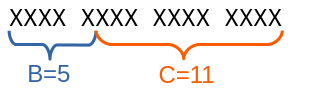
\includegraphics[scale=.5]{figures/hash.png}
  \caption{TODO nicer image.}
  \label{fig:hash}
\end{figure}

What is the probability that I am uniquely discernible (UD) in an IP
network with $Q$ hosts? I am UD if I am alone in my bucket, or if I
have strictly the greatest number of leading zeroes in my hash.
More formally:

\begin{equation}
    p(\text{Uniquely discernible}) = p(\text{Alone in bucket}) + p(\text{Most leading zeroes})
    \label{eq:highlevel}
\end{equation}

In (\ref{eq:highlevel}) there is no joint probability between the two
terms: we do not treat the case of being alone in a bucket as a special
case of having the most leading zeroes. The probability that I am alone
in a bucket when the subnet has $Q$ hosts is given by:

\begin{equation*}
    p(\text{Alone in bucket}) = \left(1-\frac{1}{2^B}\right)^{Q-1}
\end{equation*}

To figure out an expression for the second term in (\ref{eq:highlevel}),
we begin by asking ourselves ''what is the probability that I have $l$
leading zeroes in my tail?''. The tails are assumed to be uniformly
distributed bit sequences of length $C$. Then, the probability
distribution of leading zeroes is given by:

\begin{equation}
    p_L(l) =
    \begin{cases}
        \frac{1}{2^C}, & l=C \\
        \frac{1}{2^{1+l}}, & l<C \\
    \end{cases}
    \label{eq:Ldist}
\end{equation}

Next, we ask ourselves, ''given that there are a total of $N$ hashes in
my bucket, what is the probability that my $L$ is strictly the greatest
in that bucket?''. We get this from:

\begin{equation}
    p(\text{My $L$ is greatest | $N$}) = p_L(L)\left(\sum_{i=0}^{L-1}p_L(i)\right)^{N-1}
    \label{eq:domgivenN}
\end{equation}

We would like to get rid of the conditioning on $N$. To do that, we
need to know what is the probability of a bucket containing $n$ hosts.
We get that from:

\begin{equation}
    p_N(n) = \left(\frac{1}{2^B}\right)^{n-1}\left(1-\frac{1}{2^B}\right)^{Q-n}
    \label{eq:Ndist}
\end{equation}

We get rid of the conditioning by using (\ref{eq:Ndist}) to sum over
$N$ in (\ref{eq:domgivenN}):

\begin{equation}
    p(\text{My $L$ is greatest})
    = \sum_{j=2}^{Q}p_N(j)p(\text{My $L$ is greatest | $N$})
    = \sum_{j=2}^{Q}p_N(j)p_L(L)\left(\sum_{i=0}^{L-1}p_L(i)\right)^{j-1}
    \label{eq:domwithL}
\end{equation}

Notice that the outer summation starts at $j=2$ since we consider the
case of being alone in a bucket separately.

By recognising that (\ref{eq:domwithL}) contains another condition, namely
one for $L$, we realize that:

\begin{equation*}
p(\text{My $L$ is greatest})=p(\text{Most leading zeroes | $L$})
\end{equation*}

To get rid of this last conditioning on $L$, and thus obtain an expression
for the probability that I have the most zeroes in my bucket, we sum
over the different values that $L$ can take:

\begin{equation*}
    p(\text{Most leading zeroes})
    = \sum_{k=0}^{C}\sum_{j=2}^{Q}p_N(j)p_L(k)\left(\sum_{i=0}^{k-1}p_L(i)\right)^{j-1}
    = \sum_{k=0}^{C}p_L(k)\sum_{j=2}^{Q}p_N(j)\left(\sum_{i=0}^{k-1}p_L(i)\right)^{j-1}
\end{equation*}

Where $p_L$ and $p_N$ are defined in (\ref{eq:Ldist}) and
(\ref{eq:Ndist}), respectively. Thus, we see that (\ref{eq:highlevel})
depends on how we partition the hash, $B$ and $C$, and the number of
total hosts that are present in the network and it can be written as:

\begin{equation}
    p(\text{Uniquely discernible}) =
    \left(\frac{1}{2^B}\right)\left(1-\frac{1}{2^B}\right)^{Q-1} + \sum_{k=0}^{C}p_L(k)\sum_{j=2}^{Q}p_N(j)\left(\sum_{i=0}^{k-1}p_L(i)\right)^{j-1}
    \label{eq:ud}
\end{equation}

\subsection{A Small Concrete Example}
Using the parameters $Q=3$, $B=2$ and $C=2$. We calculate the probability
of becoming uniquely identifiable using (\ref{eq:ud}).

The first term is:
\begin{equation*}
    p(\text{Alone in bucket}) =
    \left(\frac{1}{2^2}\right)\left(1-\frac{1}{2^2}\right)^{3-1} \approx 0.14
\end{equation*}

